\chapter{Quantum hardware: superconducting qubits}
%\noindent
In this chapter we briefly discuss how a quantum computer is physically realized. In particular, we focus on 'superconducting qubits' that are typical quantum integrated circuit implementations which on most of the real quantum hardware are based upon since today. Firstly, we illustrate the condition a quantum computer has to satisfy and then we justify the choice of superconducting qubits. Afterwards, the most important element of such an integrated circuit, the Josephson junction, is illustrated.

It is important to underline that this chapter is only a brief introduction to the quantum hardware and that a deep analysis is beyond the aim of this thesis. 


\section{The choice of superconducting qubits}
The implementation of a real quantum hardware has to satisfy five conditions, called DiVincenzo's criteria:

\begin{enumerate}
	\item \textbf{Scalability}: system with well characterized qubit and replicable.
	\item \textbf{Reset}: ability to initialize the state of the qubits to a fiducial state as $\ket{000\dots0}$.
	\item \textbf{Long decoherence times}: the decoherence time has to be greater than the time of the execution of a circuit even more so the time of a gate application.	
	\item \textbf{'Universal' gate}: a 'universal set of quantum gate has to be provided.
	\item \textbf{Efficiently read-out}: the capability to measure the state of a qubit with a confident fidelity level.
\end{enumerate}

The main challenge of implementing a quantum hardware is to satisfy these criteria by enhancing the inter-qubit coupling while they must be at the same time completely decoupled from external influences, except during write, control and measurement phase \cite{Hardware} . Therefore, one of the main approach for implementing a quantum computer is based upon 'quantum integrated circuits', where qubits are constructed from collective electrodynamic modes of macroscopic electrical elements. The advantage is that the qubit may be coupled together via non-dissipative linear electrical elements as capacitors, inductors and transmission lines. The difficult is isolating these qubits from ambient parasitic noise. 
The first requirement for an integrated circuit, in order to behave quantum mechanically, is the absence of dissipation for all metallic parts that constituted the circuit at the qubit operating temperature. Therefore, the low temperature superconductors are the best choice for this task and such a quantum integrated circuit implementation is called '\textit{superconducting qubits}' \cite{Hardware}. The temperature of the integrated circuit has to be also less than the energy associated with the transition between the ground state, $\ket{0}$, and the excited state $\ket{1}$.%come mai?
The temperature of the wires of the control and read-out gate connected to the chip has to be low too. Quantum signal processing is performed in integrated circuit by non-linear dissipative elements that consists of superconducting tunnel junctions, also called Josephson junctions. We describe these type of junction in the following section.

%domanda: perché sono usati solo elementi non lineari per il signal processing???????????

\section{Josephson junctions}
The Josephson junctions are used in quantum integrated circuit because they are the only electronic element that are both non-dissipative (in a good approximation) and non-linear at arbitrarily low temperature \cite{Hardware}. 
It is constituted by two layers of superconducting thin films separated by an insulating layer, as illustrated in Figure \ref{junction}. The Josephson junction are based upon the tunnel effect, so the insulating layer is thin enough to allow tunneling of discrete charges through the barrier \cite{Hardware2}. In fact, at low temperatures, the superconducting films produced \textit{Cooper's pairs} that could pass trough the potential wall, originating a flux of charge flow.


\begin{figure}[h!]
\centering 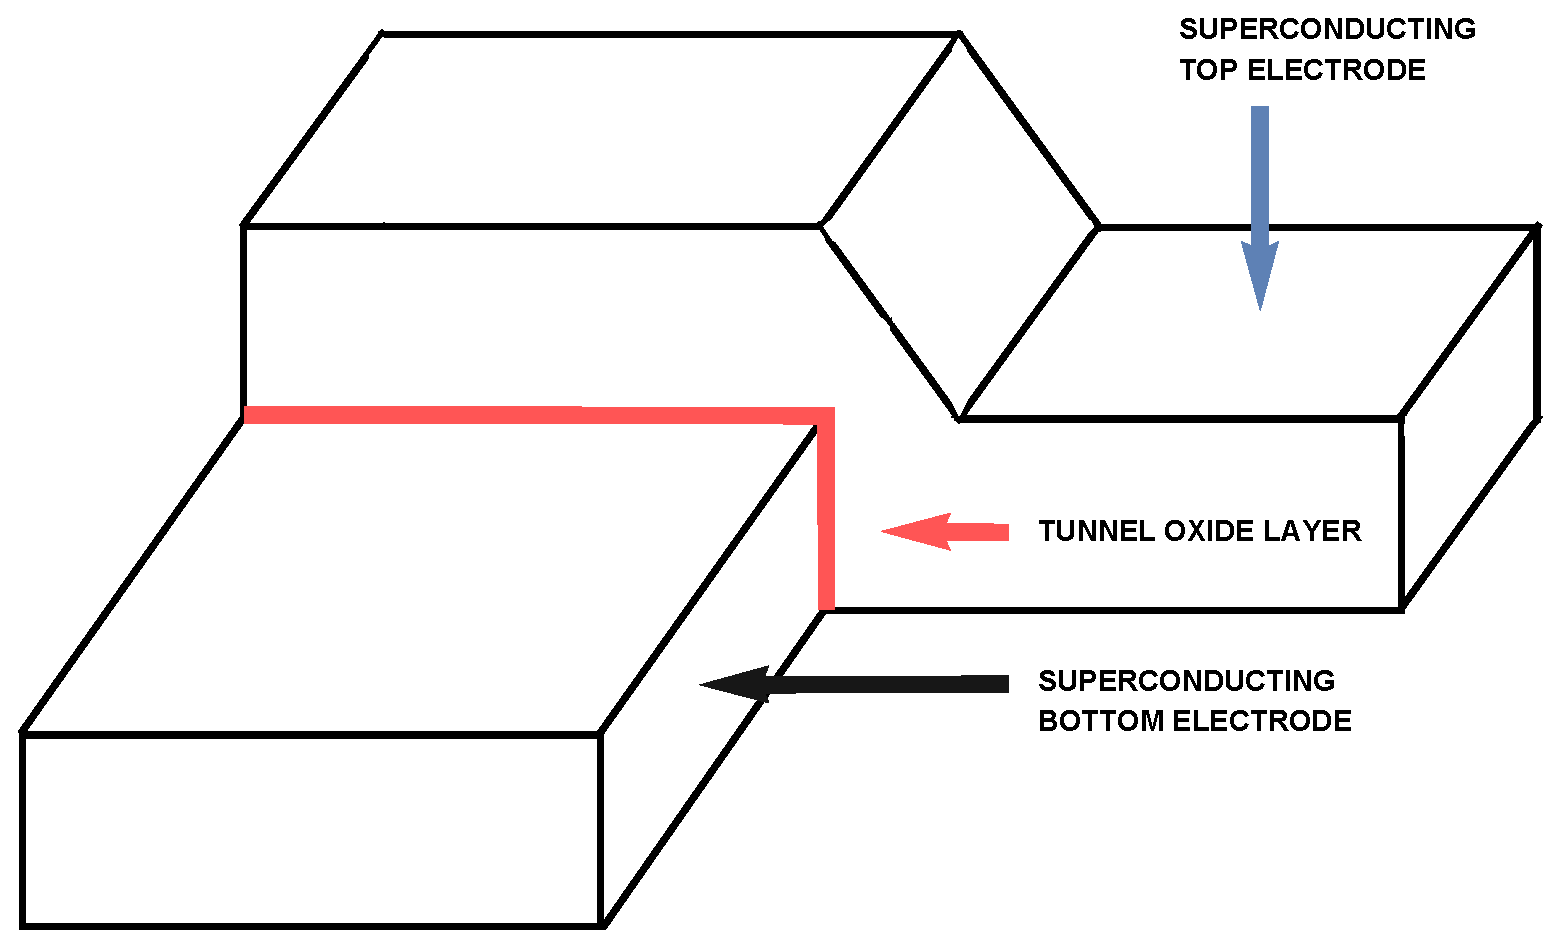
\includegraphics[width=0.5\textwidth]{./chapter4/junction.eps}
\caption{\label{junction} Josephson junction made with two superconducting thin films separated by an insulating layer that allow tunneling of discrete charges trough the barrier.  }
\end{figure}

The most simple single qubit implementation using Josephson junctions is called charge qubit.
A 'charge qubit' can be created by biasing the Josephson junction, that has an intrinsic capacity $C_J$, with a voltage source $U$ in series with a capacitor $C_G$, as shown in Figure \ref{}. The Cooper's pairs could not pass trough the capacitor shells without spending energy, therefore the superconducting layer expose to the capacitor is called \textit{island}. The junction can be described by two parameters: $N_g$, the number of Cooper's pairs in the island, and $\theta$ that is called 'superconductive phase'. The Hamiltonian of such a system is:

\begin{equation}
H= E_C (N-N_g)^2 - E_J \cos{\theta} \qquad [\theta,N] = i
\end{equation}

\noindent where $E_C=\frac{ (2e)^2}{(2(C_J+C_g))}$ is the charging energy of the island of the box ($e$ represents the electron charge) and $E_J$ is called \textit{Josephson's energy}.

\tikzset{cross/.style={cross out, draw, 
         minimum size=2*(#1-\pgflinewidth), 
         inner sep=0pt, outer sep=0pt}}
\tikzset{component1/.style={draw,thick,circle,fill=white,minimum size =0.75cm,inner sep=0pt}}
\tikzset{component2/.style={draw,thick,rectangle,fill=white,minimum size =0.75cm,inner sep=0pt}}

%%%DA MODIFICAREEE%%%


\begin{figure}[h!]
  \begin{center}
    \begin{circuitikz}[scale=0.8]
      \draw (0,0)
      to[short] (0,2)
    node[component1] {U} % The voltage source
    to[short] (0,4)
    to[C, C] (4,4) 
    to [short] (4,2)
   % \draw (3.5,2) -- (4.5,2) -- (4.5,1.5) -- (3.5,1.5) -- (3.5,2);
    node[component2] {X} 
    to[short] (4,0)
      to[short] (0,0);
    \end{circuitikz}
    \caption{}
  \end{center}
\end{figure}

The Hamiltonian could be wrote in the basis of the Cooper's pairs $\ket{N}$ as in equation \ref{HamiltonianCooper_N}, where the second term is a coupling term, that relate the state $\ket{N}$ with the state $\ket{N+1}$.

\begin{equation}
H = E_C \sum_N (N - N_g)^2 \ket{N}\bra{N} - \frac{1}{2} E_J \sum_N \ket{N+1}\bra{N} + \ket{N} \bra{N+1}
\label{HamiltonianCooper_N}
\end{equation}













